%% The following is a directive for TeXShop to indicate the main file
%%!TEX root = diss.tex

\chapter{Introduction}
\label{ch:intro}

\section{Problem Statement}
The objective of this project is to build a software which can play a wide range 
of video games. To achieve this goal, the software shall not possess any game-specific 
information. Besides, the software shall be able to play the games in a non-intrusive approach.
That is, the software shall be able to extract the necessary information 
from the screenshot of the games and control the games from standard input devices such as keyboard.
Since most of video games use graphical display as the primary interface, this requirement allows
the software to be applied to different video games.

\section{Why video games?}
Over the past decade, substantial research has been conducted to teach computer play classic strategy games such
as Deep Thought\cite{DeepBlue}, TD-Gammon\cite{Gammon}, and GO\cite{Go}.
On the other hand, little research has been made\cite{FPS}\cite{Mario} to extend the effort to other genres of video games.
The genres of video games include not only classic strategy games, but also action, first-person shooter, role-player, adventure, simulation, etc.
Video games introduce a new challenge to the AI community.

The challenge includes:
\begin{itemize}{}

\item A generic algorithm which can adapt to different types of games:
Following the paradigm of \cite{GGP} and \cite{Yavar}, the objective is not to design a good AI for
a specific game. Instead, the objective is to design a good and generic AI to play different games successfully.

\item Large but highly structured states:
For a 256 color video game with resolution $640 \times 480$, it has $256^(640 \times 480)$ states.
The number states are too big to be tractable. However, a video game often consists of small number of objects.
If we can figure out a way to represent the relationship of these objects, the number of states
can be reduced.

\item Dynamic number of agents:
Unlike classic strategy games, the number of agents in video games is highly dynamic.
The number of agents may increase over time and decrease if killed.
It is a challenge which doesn't exist in classic strategy games.
\end{itemize}

Video games can be viewed as a abstract representation of the real world. Often can we find the 
correspondence between such an artificial world to a real-world problem\cite{KeepAway}.
Focusing on Video games allows us to attack a real-world problem without tackling unnecessary details, while maintaining sufficient 
level of abstraction. In addition, video games are well-understood and customizable environments. 
It allows us to test an AI algorithm and justify if the result is correct\cite{Yavar}.

Another possible application is the AI of video games.
Nowadays, the AI engineers usually need to craft the behavior of AI by hand. 
The process are time-consuming and the hard-coded behavior would produce unrealistic AI behavior.
If we can design a generic agent and let it act reactively with the environment, it can produce 
more various and unpredictable behaviors.

\section{Why applying computer vision to video games?}

The reason behind is the reality that most of the video games do not have source codes which are publicly available.
If a researcher needs to test his algorithm on Super Mario Bros., all he can do is to apply it on Infinite Mario Bros.,
which is an open source clone of original Super Mario Bros. He cannot test his algorithm on Mario Bros. 1 or 2, which are available
on binary format. If a researcher does not have source codes, he cannot extract the game states like the location
of Koopa Troopas which are mandatory for any AI algorithm to work. 

Using computer vision techniques to extract the information from the game screen is a way to solve this problem.
Because most of the video games uses graphics as the primary interface to interact with the player, it contains
the necessary information for the player to play. The use of computer vision allows us to test the algorithm
non-intrusively, without the effort to hack the game engine or reimplement the game.

Besides, the vision allows a more generic way for a computer to play a video game. It creates 
new applications which cannot be done by intrusive approaches.

\begin{itemize}{}
\item Non-intrusive and generic AI:
Have you ever played a good game with poor AI? Can you change it with a better one?
Without the source codes of the game or the engine support, the answer is usually "No".
Nevertheless, if we could design a software which can learn to play any video game, 
the answer can be changed to "Yes". The non-intrusive and generic agents can be 
applied to any video games with/without the support from the game company.

\item Modding: 
Game modding becomes popular in recent years \cite{Modding}. 
Modding allows users to customize the video games to suite their personal tastes.
The modding usually includes the introduce new content, modification of original one, or remove the unsatisfactory elements.
The process can be done by the support of game development kit released by the game company.
It can also be done without the support from the game company. However, the modders need to hack the game engine,
decode the data format and implement their own development kit. 
The process can be time-consuming and tedious.
If we could automate the process by having a software which can 
traverse the game and extract the in-game elements for us, it could save a lot of time.

\end{itemize}

%\chapter{Related Work}
%\label{ch:Related}
\section{Related Work}

There are several works which address how to design a good AI for certain type of video games.
McPartland et al. proposed a approach to allow bots in First-Person Shooter (FPS)
games to learn how to navigate the maze and handle combat \cite{FPS}. M. Smith et al. proposed a coordination 
framework to allow the bots to adapt to different strategy by reinforcement learning \cite{FPS_TEAM}. 
Michael et al. applied a Monte Carlo planning approach for Real-Time Strategy (RTS) gmaes to 
the Rush-the-Flag game \cite{RTS}. Ponsen et al. proposed hierarchical relational learning to learn how to play
the Battle of Survival game \cite{HRRL}. For arcade-style games, \cite{Mario} uses a RL agent to learn
how to play Infinite Mario Bro. Driessens et al. proposed a relational RL to learn how to play the Digger
game. In \cite{OO}, a object-oriented representation is proposed to play pitfall.

Previous works rely on the intrusive approach to provide the states of games for the agents to play.
The agents need to know the information such as the number of objects, the types of objects,
or the health level of players to play the games. The intrusive approach makes it difficult to generalize
to a large number of video games. And the game-specific representation prevents these approaches
to be applied to arbitrary video games.

With the objective to play general video games, our work is most related to 
General Game Playing\cite{GGP} (GGP) and Playing Atari 2600 \cite{Yavar}. 
The objective of GGP is to develop a software agent which can play unspecific games if the rules
are given. Our work follows the same objective. However, due to the complexity of video games, 
it is not clear that how to precisely describe the rules of video games.

Y. Naddaf\cite{Yavar} proposed A.L.E. (Atari 2600 Learning Environment) as the platform to test AI algorithms.
A.L.E. supports fast emulation and generic interface. Fast emulation allows the emulator to run 
games without rendering or sound generation. It can increase the speed in the learning phase.
The generic interface provides AI agents the screenshot and scores in games. It allows us
to build the agents in a game independent way.

Our work is built on A.L.E. However, our work differs from \cite{Yavar} in the following perspective:

\begin{itemize}{}
\item Our work features object-based representation. We argue that objects are the fundamental elements
in video games. The representation allows the agent to develop appropriate policy against specific 
objects. And it also enables the possibility to reuse the knowledge in different stages.
\end{itemize}

\chapter{Reinforcement Learning}
\label{ch:RL}
The objective of reinforcement learning algorithm is to build a learning agent. The learning agent will take
actions based on the current state. In the beginning, the agent does not know anything about 
the environment, therefore the agent has to choose the first action randomly. After the environment
receives the action, it will provide a reward to the agent as a feedback. The reward can be either
positive or negative.

The agent adjusts the value function to maximize the expected reward in the future.
The value function represent the expected reward when the agent takes certain action in the current
state, and it is used to estimate the "quality" of an action. The initial value of value function is 
usually 0, but it is possible to set it to some high enough value to encourage exploration.
It is important to evaluate the value function 
correctly. If some actions with low expected reward are estimated as high, it degrades the
performance of agent.

The agent can select an action which leads to the highest value of value function. However, 
this strategy does not allow the agent to explore the states which are not visited before.
A better approach is to use $\epsilon$-greedy method. The method allows the agent to abandon the
best action and choose
a random action with a very small probability $\epsilon$. The higher the probability, the more
likely that the agent would explore the new actions. However, if the exploration probability 
is too high, it will increase the time to converge.

After the agent takes an action, the environment will provide a reward and a state to the
agent. The agent then decides an new action for the new state. After several iterations
, the agent will learn a correspondence between the action and state. The correspondence is called 
"policy". 

\section{Temporal Difference}
\label{sec:TD}
There are 3 types of reinforcement learning algorithms -- dynamic programming(DP), Monte Carlo 
methods, and temporal-difference (TD). Dynamic programming can compute the optimal policy, but it 
requires a precise model of the environment. In most of the cases, the environment
is too complex to be modeled precisely, and it is not easy to get the complete information about
the environment. On the other hand, it is usually possible to use Monte Carlo method to sample the environment to
get the partial information. 
Like Monte Carlo method, TD uses sampling, therefore it does not require the 
complete model of the environment. TD method is a bootstrapping method, similar to the dynamic 
programming approach, it updates the new value function based on the previous one.

The equation to compute the value function in TD:
\begin{displaymath}
   V(S_t) \leftarrow V(S_t) + \alpha [r_{t+1} + \gamma V(S_{t+1}) - V(S_t)],
\end{displaymath}

where $V(s_t)$ is the value function of the state $s_t$. $V(s_t)$ is the expected reward when
the agent reaches the state $s_t$. $r_{t+1}$ is the reward given to the agent when it chooses
the action at state $s_t$.

\section{SARSA}
\label{sec:SARSA}
SARSA is a on-policy TD approach. On-policy indicates that it learns from the current policy.
Different from other TD approaches, SARSA updates the Q value of the current state-action from the next state-action.
The Q value is updated by:
\begin{displaymath}
    Q(s_t, a_t) \leftarrow Q(s_t, a_t) + \alpha [r_{t+1} + \gamma Q(s_{t+1}, a_{t+1})-Q(s_t, a_t)],
\end{displaymath}
where $Q(s, a)$ is the value function for state-pair, and it is the expected reward when the agent takes
the action $a$ at the state $s$. $\alpha$ is step-wise, which controls the learning rate. 
$\gamma$ is the discount factor.


\begin{center}
\begin{tabular}{@{}lp{6cm}@{}}
\hline
Algorithm: SARSA\\
\hline
Initialize $Q(s, a)$ arbitrarily\\
Repeat (for each episode)\\
\ \ \ \ \ \ Initialize $s$\\
\ \ \ \ \ \ Choose $a$ based on $s$ using policy derived from $Q$ (e.g., $\epsilon$-greedy method)\\
\ \ \ \ \ \ Repeat (for each step of episode):\\
\ \ \ \ \ \ \ \ \ \ \ \ Take action $a$, obtain reward $r$ and next state $s'$ from the environment\\
\ \ \ \ \ \ \ \ \ \ \ \ Choose $a'$ based on $s'$ using policy derived from $Q$ (e.g., $\epsilon$-greedy method)\\
\ \ \ \ \ \ \ \ \ \ \ \ $Q(s, a) \leftarrow Q(s, a) + \alpha [r + \gamma Q(s', a')-Q(s, a)]$\\
\ \ \ \ \ \ \ \ \ \ \ \ $s \leftarrow s'$\\
\ \ \ \ \ \ \ \ \ \ \ \ $a \leftarrow a'$\\
\ \ \ \ \ \ Until $s$ is terminal\\
\hline  
\end{tabular}
\end{center}

\section{Q-Learning}
\label{sec:Q-Learning}
    Q-Learning is an off-policy TD approach. Compared to SARSA, Q-Learning updates
the Q value by the highest value of the next possible state-action, rather than the 
next state-action executed by the agent.  
The Q value is updated by:
\begin{displaymath}
   Q(s_t, a_t) \leftarrow Q(s_t, a_t) + \alpha [r_{t+1}+\gamma \max_a Q(s_{t+1},a)-Q(s_t,a_t)],
\end{displaymath}

where $\max_a Q(s_{t+1},a)$ is the highest value of the next possible state-action. 


\begin{center}
\begin{tabular}{@{}lp{6cm}@{}}
\hline
Algorithm: Q-Learning\\
\hline
Initialize $Q(s, a)$ arbitrarily\\
Repeat (for each episode)\\
\ \ \ \ \ \ Initialize $s$\\
\ \ \ \ \ \ Repeat (for each step of episode):\\
\ \ \ \ \ \ \ \ \ \ \ \ Choose $a$ based on $s$ using policy derived from $Q$ (e.g., $\epsilon$-greedy method)\\
\ \ \ \ \ \ \ \ \ \ \ \ Take action $a$, obtain reward $r$ and next state $s'$ from the environment\\
\ \ \ \ \ \ \ \ \ \ \ \ $Q(s, a) \leftarrow Q(s, a) + \alpha [r + \gamma max_{a'} Q(s', a')-Q(s, a)]$\\
\ \ \ \ \ \ \ \ \ \ \ \ $s \leftarrow s'$\\
\ \ \ \ \ \ Until $s$ is terminal\\
\hline  
\end{tabular}
\end{center}

\section{minmax Q-Learning}
\label{sec:minmax}

    In two player zero-sum game, it's reasonable to take the action of the opponent into consideration.
In minmax Q-learning, the Q value is a function of state, the action of player, and the action of opponent.
The Q value is updated by:
\begin{displaymath}
    Q(s_t, a_t, o_t) \leftarrow Q(s_t, a_t, o_t) + \alpha [r_{t+1}+\gamma\max_a min_o Q(s_{t+1}, a, o)-Q(s_t, a_t, o_t)],
\end{displaymath}

\begin{center}
\begin{tabular}{@{}lp{6cm}@{}}
\hline
Algorithm: minmax Q-learning\\
\hline
\ \ \ Initialize: $Q(s, a, o) \leftarrow 1, V(s) \leftarrow 1$
\ \ \ Repeat (for each episode)\\
\ \ \ \ \ \ Initialize $s$\\
\ \ \ \ \ \ Repeat (for each step of episode):\\
\ \ \ \ \ \ \ \ \ \ \ \ Choose $a$ based on $s$ using policy derived from $Q$ (e.g., $\epsilon$-greedy method)\\
\ \ \ \ \ \ \ \ \ \ \ \ Take action $a$, obtain opponent action $o$, reward $r$ and next state $s'$ from the environment\\
\ \ \ \ \ \ \ \ \ \ \ \ $Q(s, a, o) \leftarrow Q(s, a, o) + \alpha [r + \gamma max_{a'} min_{o'} Q(s', a', o')-Q(s, a, o)]$\\
\ \ \ \ \ \ \ \ \ \ \ \ $s \leftarrow s'$\\
\hline  
\end{tabular}
\end{center}


\chapter{Relational Reinforcement Learning}

Video games involves objects: things like monsters, treasures, or princess.
The game world can be described by the relation of objects: there is a
beautiful princess who is prisoned in a castle which is guarded by a horde of
monsters.  When we play the game, it is more nature to consider an action in a
relational form. Are there any monsters near the treasure?  How many monsters
are in the next room?  The states and actions in video games can be more
effectively to be represented in relational forms. 

Reinforcement learning provides a general approach to construct an intelligent
agent with minimal supervision. Nevertheless, most work in reinforcement
learning focuses on propositional representations. Such representation requires
some human expert to construct a fixed-length feature vector to represent the world.
However, it is difficult to construct a fixed-length feature vector to
represent varying number of monsters in video games.
%It is also not clear how to assign each monster to the corresponding feature.
In addition, the
relationships between objects are lost in the propositional representation,
unless it is hand-crafted into the feature vector by the human expert. The lack
of object information makes it hard to transfer the knowledge against one class
of objects to against another similar one. 

The insufficient power of propositional representation motivates the relational
reinforcement learning algorithms.  
The relational reinforcement learning can be formulated as Relational Markov Decision Process (RMDP).


%Dynamic number of objects
%No fixed representation
%Dependency with samples. (intrinsic to reinforcement learning, since consective states has similar
%Q-value, there are not independent all)

%But the most current machine learning algorithms requires the world to be represented 
%by a vector of attributes. The vector representation has several drawbacks when applied to objects.


%The vector representation is ordered. However, it's not clear how to assign a fixed for the objects.

%The length of vector representation is fixed. However, the number of objects might vary.

%The relationship between objects are lost in the vector representation. 

%\section{Object-Oriented Relational Reinforcement Learning}
\section{Relational Markov Decision Processes}

Following the definition in \cite{RelationalMDP}, we define 
a relational MDP as follows:

%TODO: Add normal Definition here
Definition: Relational Markov decision process (RMDP) is formalized as a tuple $<P_S, P_A, C, T, R>$, where
\begin{itemize}{}
\item $P_S$ is a set of state predicates.
\item $P_A$ is a set of action predicates.
\item $C$ is a set of object classes. 
\item A state $S$ in state space $\mathbb{S}$ is a set of state predicates.
\item A action $S$ in state space $\mathbb{S}$ is a set of state predicates.
\item The transition function $T:S \times A \times S \rightarrow [0, 1]$ defines a probability distribution over the possible next states. 
\end{itemize}

%To solve the RMDP, common approaches involve relational regression and approximate policy iteration.
%Example: Mario Coin Monster world
%The example state, action, 
%The propositional representation {(1, 24, 3), (2, 35, 6)}
%input is a tuple
%The common approach to solve the RMDP problem
%Feature Engineering
%Relational Regression
%Approximate Policy Iteration

\begin{figure}[h]
    \centering
    \begin{minipage}[t]{0.6\linewidth}
        \centering
        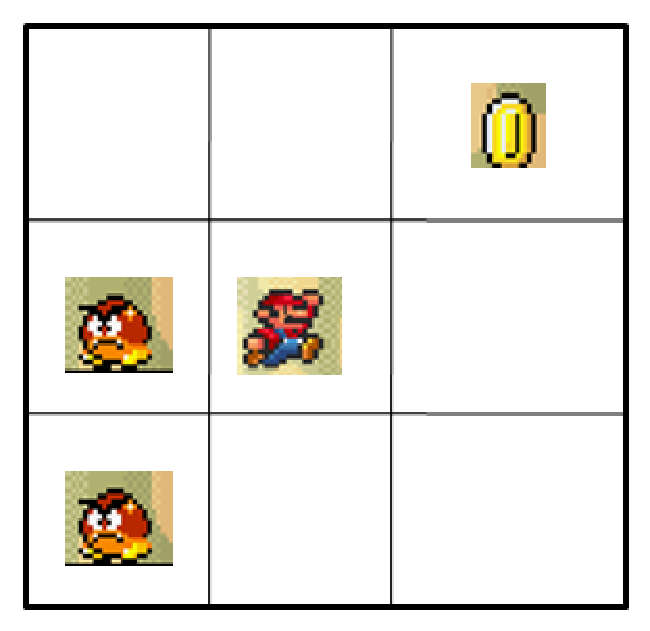
\includegraphics[width=\textwidth] {./figures/MarioWorld.eps}
        \caption{The world with two monsters $M1$ and $M2$. A coin and a agent.}
    \label{fig:MarioWorld}
    \end{minipage}
\end{figure}


Motivated by \cite{RelationalTemplate} and \cite{RelationalMDP}, we decompose the value function into
into the summation of several local functions, which are defined over some templates. 
Each template represents a policy against a certain type of object.

For example, the world in fig. \ref{fig:MarioWorld} consists of an agent, a
coin and two monsters.  The agent gets +10 reward when he picks a coin and
receives -10 reward if he encounters a monster.  The value function of the
agent can be represented as $V = V_{monster}(A, M1) + V_{monster}(A, M2) +
V_{coin}(A, C)$.  The location functions $V_{monster}$ and $V_{coin}$ indicates
the expected rewards when there is one such object in the world. The
decomposition of value function allows us to handle varying number of objects
by summation over local functions. The class-specific location function also
allows to share the knowledge from different objects of the same type. 
The agent knows how to handle a new entity if the agent has experience of the same type
before. In other worlds, the location functions enable knowledge transfer with in the 
same class.

%To learn the local value function, we 

It motivates the following relational template Q-Learning algorithm:
%My solution
\begin{center}
\begin{tabular}{@{}lp{6cm}@{}}
\hline
Algorithm: relational template Q-Learning\\
\hline
Initialize $Q(s, a)$ arbitrarily\\
Repeat (for each episode)\\
\ \ \ \ \ \ Initialize $s$\\
\ \ \ \ \ \ Repeat (for each step of episode):\\
\ \ \ \ \ \ \ \ \ \ \ \ Choose $a$ based on $s$ using policy derived from $Q$ (e.g., $\epsilon$-greedy method)\\
\ \ \ \ \ \ \ \ \ \ \ \ Take action $a$, obtain reward $r$ and next state $s'$ from the environment\\
\ \ \ \ \ \ \ \ \ \ \ \ For each object $O_i$:\\
\ \ \ \ \ \ \ \ \ \ \ \ \ \ \ \ \ \  $Q_{C_i}(s, a) \leftarrow Q_{C_i}(s, a) + \alpha [r + \displaystyle\gamma \  max_{a'} Q_{C_i}(s', a')-Q_{C_i}(s, a)]$\\
\ \ \ \ \ \ \ \ \ \ \ \ $Q(s, a) = \displaystyle\sum_{i} Q_{C_i}(s, a)$\\
\ \ \ \ \ \ \ \ \ \ \ \ $s \leftarrow s'$\\
\ \ \ \ \ \ Until $s$ is terminal\\
\hline  
\end{tabular}
\end{center}

%update by Q by local value function or the global one? (which one will converge faster?)
%context independent ??

%Weakness of current approach
%TG uses a big classification tree to learn all policy of the agent in its lifetime, we need a new way to find the policy against local structure, for transfer
%

%Handle dynamic number of objects (what if a class is missing?) what is the regression tree work?
%Learn simple scenario from complex one--
%Peter Stone's soccer need a simple scenario to transfer
%But in video games we cannot do it
%Current approach cannot transfer from complex one to simple one, how can it be done? From two block to three blocks
%Hanlde real value relations
%Implement the current approach
%the system dynamics and rewards

%spatial proximity
%temporal proximity
%structure learning, group small number of objects into bigger one (CVPR 2010, Yu Pen Fei's project)









































\endinput
at the level of a template for a task domain. Given a particular
environment within that domain, it defines a specific MDP
instantiated for that environment. The domain is specified by a schema,
which specifies a set of object classes C = fC1; : : : ;Ccg. Each class
C is also associated with a set of state variables S[C] =
fC:S1; : : : ;C:Skg, which describe the state of an object in
that class. Each state variable C:S has a domain of possible
values Dom[C:S]. We define SC to be the set of possible
states for an object in C, i.e., the possible assignments to the
state variables of C.
For example, our Freecraft domain might
have classes such as Peasant, Footman, Gold;
the class Peasant may have a state variable
Task whose domain is Dom[Peasant:Task] =
fWaiting, Mining, Harvesting, Buildingg, and a state
variable Health whose domain has three values. In this
case, SPeasant would have 4  3 = 12 values, one for each
combination of values for Task and Health.
The schema also specifies a set of links L[C] =
fL1; : : : ;Llg for each class representing links between objects
in the domain. Each link C:L has a range [C:L] = C0.
For example, Peasant objects might be linked to Barrack
objects — [Peasant:BuildTarget] = Barrack, and to the
global Gold and Wood resource objects. In a more complex
situation, a link may relate C to many instances of a
class C0, which we denote by [C:L] = fC0g, for example,
[Enemy:My Footmen] = fFootmang indicates that an instance
of the enemy class may be related to many footman instances.
A particular instance of the schema is defined via a
world !, specifying the set of objects of each class; we use
O[!][C] to denote the objects in class C, and O[!] to denote
the total set of objects in !. The world ! also specifies
the links between objects, which we take to be fixed
throughout time. Thus, for each link C:L, and for each
o 2 O[!][C], ! specifies a set of objects o0 2 [C:L], denoted
o:L. For example, in a world containing 2 peasants,
we would have O[!][Peasant] = fPeasant1;Peasant2g;
if Peasant1 is building a barracks, we would have that
Peasant1:BuildTarget = Barrack1.
The dynamics and rewards of an RMDP are also defined
at the schema level. For each class, the schema
specifies an action C:A, which can take on one of several
values Dom[C:A]. For example, Dom[Peasant:A] =
fWait, Mine, Harvest, Buildg. Each class C is also associated
with a transition model PC, which specifies the probability
distribution over the next state of an object o in class
C, given the current state of o, the action taken on o, and the
states and actions of all of the objects linked to o:
PC(S0
C j SC;C:A;SC:L1 ;C:L1:A; : : : ;SC:Ll ;C:Ll:A): (1)
For example, the status of a barrack, Barrack:Status0,
depends on its status in the previous time step, on
the task performed by any peasant that could build it
(Barrack:BuiltBy:Task), on the amount of wood and gold, etc.
The transition model is conditioned on the state of C:Li,
which is, in general, an entire set of objects (e.g., the set of
peasants linked to a barrack). Thus we must now provide
a compact specification of the transition model that can depend
on the state of an unbounded number of variables. We
can deal with this issue using the idea of aggregation [10].
In Freecraft, our model uses the count aggregator ], where
the probability that Barrack:Status transitions from Unbuilt to
Built depends on ][Barrack:BuiltBy:Task = Built], the number
of peasants in Barrack:BuiltBy whose Task is Build.
Finally, we also define rewards at the class level. We assume
for simplicity that rewards are associated only with the
states of individual objects; adding more global dependencies
is possible, but complicates planning significantly. We define
a reward function RC(SC;C:A), which represents the contribution
to the reward of any object in C. For example, we
may have a reward function associated with the Enemy class,
which specifies a reward of 10 if the state of an enemy object
is Dead: REnemy(Enemy:State = Dead) = 10. We assume
that the reward for each object is bounded by Rmax.
Given a world, the RMDP uniquely defines a ground factored
MDP !, whose transition model is specified (as usual)
as a dynamic Bayesian network (DBN) [3]. The random variables
in this factored MDP are the state variables of the individual
objects o:S, for each o 2 O[!][C] and for each
S 2 S[C]. Thus, the state s of the system at a given point in
time is a vector defining the states of the individual objects in
the world. For any subset of variablesX in the model, we define
s[X] to be the part of the instantiation s that corresponds
to the variables X. The ground DBN for the transition dynamics
specifies the dependence of the variables at time t+1
on the variables at time t. The parents of a variable o:S are
the state variables of the objects o0 that are linked to o. In our
example with the two peasants, we might have the random
variables Peasant1:Task, Peasant2:Task, Barrack1:Status,
etc. The parents of the time t + 1 variable Barrack1:Status0
are the time t variables Barrack1:Status0, Peasant1:Task,
Peasant2:Task, Gold1:Amount andWood1:Amount.
The transition model is the same for all instances in the
same class, as in (1). Thus, all of the o:Status variables for

Health H’

Count
   	 
Health H’
AFootman

 
F1.Health
F1.A
F1.H’
E1.Health E1.H’
F2.Health
F2.A
F2.H’
E2.Health E2.H’

������



 	 
 
 	 
 

Time   
(a) (b)
Figure 2: Freecraft tactical domain: (a) Schema; (b) Resulting factored
MDP for a world with 2 footmen and 2 enemies.
barrack objects o share the same conditional probability distribution.
Note, however, that each specific barrack depends
on the particular peasants linked to it. Thus, the actual parents
in the DBN of the status variables for two different barrack
objects can be different.
The reward function is simply the sum of the reward functions
for the individual objects:
R(s; a) = X
C2C
X
o2O[!][C]
R(s[So]; a[o:A]):
Thus, for reward function for the Enemy class described
above, our overall reward function in a given state will be
10 times the number of dead enemies in that state.
It remains to specify the actions in the ground MDP. The
RMDP specifies a set of possible actions for every object in
the world. In a setting where only a single action can be taken
at any time step, the agent must choose both an object to
act on, and which action to perform on that object. Here,
the set of actions in the ground MDP is simply the union
[o2!Dom[o:A]. In a setting where multiple actions can be
performed in parallel (say, in a multiagent setting), it might
be possible to perform an action on every object in the domain
at every step. Here, the set of actions in the ground MDP is a
vector specifying an action for every object: o2!Dom[o:A].
Intermediate cases, allowing degrees of parallelism, are also
possible. For simplicity of presentation, we focus on the multiagent
case, such as Freecraft, where, an action is an assignment
to the action of every unit.
Example 2.1 (Freecraft tactical
Any text after an \endinput is ignored.
You could put scraps here or things in progress.

Objective: Allow computer to play video games
Objective2: perfect modeling
abundance of old games
home robot entertaunnent(kinetics) join the family
Approach:
Input: Screen and Reward function
1. Video Analysis 
2. Control the game by RL algorithms--RL algorithms must be able to be applied to different games successfully
3. Modeling dynamics(the agent needs to explore the game to get enough information)

Comparison to previous work:
1. Nonintrusive gaming(compared to NIPS 2008)
2. Modeling the game
Chanllenge:
1. Real-Time Video Anaylysis
2. A generic RL algorithm which works on different games
Unlike previous work on RL, the objective is not to design a good AI for a specific game to against
human player, the objective is to design a good and generic AI for play different games successfully
But it is not required to be perfect or optimal. AI in video games cannot be perfect, otherwise it 
would be not possible for a human player to beat the game. The opponent is suboptimal in nature.
3. Little prior knowledge on the games. Unlike keep away, it's not possible to design heiracial action
for (Pong). It must be able to play the game from primitive actions or construct the complex actions by itself.
Volleyball
Example: 
  Fireball vs Soccer ball
  In one game, it's necesart to intercept the soccer ball.
  In another game, it's lethal to touch any ball.
4. Huge game states(640X480X30X(256) per seconds), highly redudunet
5. Little training time (the game has 30fps), cant increase that
6. Dynamic number of agents(avoid ball)(different from soccer)(the number of player is dynamics (unlike game theory))

Motivation for reinforcement learning

Articial Intelligence algorithms that can play classic or video games have been studied ex-
tensively. Research in classic games has resulted in Deep Thought for chess [Campbell et al., 2002],
Chinook for checkers [Schaeer et al., 2005], TD-Gammon for backgammon [Tesauro, 1994],
and Polaris for poker [Bowling et al., 2009]. For AI researchers who work on solving vari-
ous games, there is a recurring question that needs to be addressed: why dedicate limited
resources to solving games instead of tackling the real-world problems in which the eld of
Articial Intelligence can contribute to the daily quality of human lives? In other words,
why spend resources on solving chess, if what we need is self-driving cars with near zero
collision rates? Why play checkers, if what we want is an intelligent maid robot that can
cook, vacuum, and wash the dishes?
The motivation for developing AI agents that can play games is threefold. First, games
oer controlled, well-understood, and easily abstracted environments, with well-dened mea-
sures of success and failure. These properties make games suitable platforms for developing
and testing AI algorithms. The methods developed and the knowledge gained from work-
ing in these controlled environments can later be applied to the real-world problems which
are generally messier and harder to measure performances, but still require the same AI
sophistication.
Additionally, games are excellent platforms for showcasing the capabilities of the latest
AI techniques to the public. In 1997, when Deep Blue defeated Garry Kasparov, a great
wave of excitement was generated among regular, non-academic people about Articial
Intelligence. This is because people understand chess, and respect the complexity involved
in playing it well. Back in 1997, the AI community was not able to develop collision-free
autonomous cars or achieve many other longer-term goals of the eld. Showcasing an agent
that mastered chess helped the public understand what the AI community was capable of
at the time.
Finally, with the recent growth of commercial video games into a multibillion-dollar
industry, there is now even more motivation for studying agents that can learn to act intelli-
gently in games [Lucas, 2009, Laird and Lent, 2000]. Non-repetitive, adaptive, interesting,
and in summary intelligent behavior oers a competitive edge for commercial games. As
the game graphics peak at image-like quality, and as the game consoles oer more and more
computational power that can be spent on complex learning algorithms, the importance of
3


Application:
1. desktop (sort the data row??)
2. gaming ( a alternative of in game AI) can act as opponent or friends (human and computer cooperation)( with 2 different computers)
3. game modeling ( convert to another platform)
2. simulatioin env forj robot
4. agent in online gaming (need to go to toilet)
5. General in game AI
6. General in computer sceice (viki, robot soccer simulated)

high level editing
4. game synthesys (chane the protagonist in game, add monsters)

Problem Statement
The objective of this project is to build a software which can play a wide range 
of video games. To achieve this goal, the software shall not possess any game-specific 
information. Besides, the software shall be able to play the games in a non-intrusive approach.
That is, the software shall be able to extract the necessary information 
from the screenshot of the games and control the games from standard input devices such as keyboard.
Since most of video games use graphic display as the primary interface, this requirement allows
the software to be applied to different video games.

Why video games?
Go beyond Chess and robot soccer:
Over the past decade, substantial research has been conducted to teach computer play classic strategy games such
as Deep Thought for chess [Campbell et al., 2002],
Chinook for checkers [Schaeer et al., 2005], TD-Gammon for backgammon [Tesauro, 1994],
go (Silver, Sutton, and Muller 2007).
and Polaris for poker [Bowling et al., 2009].
On the other hand, little research has been made [cite here] to extend the effort to other genres of video games.
The genres of video games include not only classic strategy games, but also action, first-person shooter, role-player, adventure, simulation, etc\ldots
These games introduce the new challendge to AI community
Complex, can have really large, continuous state and
action spaces.

Can we go beyond the classic ones to investigate the more diversifying video games? 

But why do we need to study suce a topic?
Nowadys, it's quite normal for game company to 
Video games can be viewed as a abstract representation of the real world. Often can we find the 
correspondence between such an ariticial world to a real-world problem<robot soccer, viki>.
Video games allow us to attack a real-world problem without tackling uncessary details, while maintaing enough 
level of abstraction.
Video games are well-understood, custimizable environments. They allow us to work test an AI algorithm
and justify if the result is correct. <alberta, Namir>

Another application is the game industry.
Nowadys, the AI engineers usually need to craft the behavior of the AI by hand. 
The process are time-comsuing and it will produce unrealistic charactor behavior.
If we can design 

Educational


Why vision on video games?

The reason behind is based on the reality that most of the video games do not have source codes publicly available.
If a researcher needs to test his RL alogrithm on Super Mario Bros., all he can do is to apply it on (infinity mario),
since it's the only Mario which goes open source. He cannot test his alrogithm on Mario 1 or 2, which are availbel
on binary. If a researher does not have a source code, he cannot extract the game state like the locaiton
of scoobma which are mandatory for any AI alogrithm. 

Using computer vision techniques to extract the information from the game screen is a way to solve this problem,
since most of the video games uses graphics as the primary interface to interact with the player, it contains
the necessary information for the player to play. The use of computer vision allows us to test the algorithm
non-intrusively, without the effort to hack the game engine or reimplement the game.

Besides, the vision allows a more generic way for a computer to play a video game. It creates 
new applications which cannot be done by intrusive approaches.

Nontrusive and generic AI:
Have you ever experience a good game with poor AI.

--------------High level modeling---------------------
Modding: 
Game modding becomes popular in recent years [modding], 
Modding allows users to customize the video games to suite their personal tastes.
The modding usually includes the introduce new content, modification of oringinal ones, remove the unsatisfactory elements.
The process is usually can be done by the support of game developement kit released by the game company.
It can also be done without the support from the game company. The players need to hacking the game engine,
to decode the data format and develope their own developlment kit. 
Eductional part: --> put the education effort to the game without engine support
It enables the possibility of Nonintrusive modding.
Reuse the AI module in other games. Reuse the content from other games

One engine rules all
In previous, video games are built from scratch. A game company first decides the types of the game,
then then developed the game engine and the content of the game. Later, people starts to figure out 
that the game engine and the content of the game can be separated. The content of the game mostly consist of
artistic materials, dialogs and simple scripte, while the game engines handle the most programming part.
To the game engine, the content is nothing but a set of data. It's more efficient to reuse the same enging
to create multiple games. The reconigction creates the game company which specialized in content, while other
focused on the content. I 
The game companies usually .
Is it possible to use one engine to run all video games?
It is a distinct dream, and cannot be done by policital force.
The modeling of video games also allows us to convert abitrary game into
some unified represention such UML. 
With the universial representation,
it creates the possibility to use one game engine, which serve as the interpret of the content, to run all video games.

It is a dream
The modeling of video games also create the possibility to use 
Platform indepent description of a video game:
There are abunadnt of old games which can 
One simulator for all games
mobile platform: iphone, gphone
web appl: play it on line flash

The modeling of the video games allows us to extract the graphics, the dynamics
and the AI in video games. It enables the possibility to reconstruct the game in 
a high level way. 
--------------High level modeling---------------------


allows the users to modify the 

There has been a recent increase in the number of game environments or engines
that allow users to customize their gaming experiences by building and
expanding game behavior. This article describes the use of modifying, or
modding, existing games as a means to learn computer science, mathematics,
physics, and aesthetic principles. We describe two exploratory case studies of
game modding in classroom settings to illustrate skills learned by students as
a result of modding existing games. We also discuss the benefits of learning
computer sciences skills


Entertainment and Educational Robot:
In the future, 
The robots are not only for chores, it will become a part of the family.
It can listen, and speak with people. 
It won't be a machine which can only execute the instruction from people.
It will give feedback to the poeple. Tell poeple the solution.
It will have be emotionally connected with people.
Teach the young generation how to use computers. 
A future that human and robot can work together and play together.
The possbility shall not be limited to physical games, but also video games.
How can a computer learns how to use another computer.

There will be emotional connection with the robots and people. 

It can play with child,
teach people how to use computer, or even play video games. 
production or domestic services





Computer vision 
1. no source code
Modding
Remodoling
Nonintrusive AI (in different computer)
Gaming robot(Teach people use computer family member, play with people, home robot not chores)
2. have source code, but hard to modify
A general way to manupulate program
3. 



Articial Intelligence algorithms that can play classic or video games have been studied ex-
tensively. Research in classic games has resulted in  For AI researchers who work on solving vari-
ous games, there is a recurring question that needs to be addressed: why dedicate limited
resources to solving games instead of tackling the real-world problems in which the eld of
Articial Intelligence can contribute to the daily quality of human lives? In other words,
why spend resources on solving chess, if what we need is self-driving cars with near zero
collision rates? Why play checkers, if what we want is an intelligent maid robot that can
cook, vacuum, and wash the dishes?
The motivation for developing AI agents that can play games is threefold. First, games
oer controlled, well-understood, and easily abstracted environments, with well-dened mea-
sures of success and failure. These properties make games suitable platforms for developing
and testing AI algorithms. The methods developed and the knowledge gained from work-
ing in these controlled environments can later be applied to the real-world problems which
are generally messier and harder to measure performances, but still require the same AI
sophistication.
Finally, with the recent growth of commercial video games into a multibillion-dollar
industry, there is now even more motivation for studying agents that can learn to act intelli-
gently in games [Lucas, 2009, Laird and Lent, 2000]. Non-repetitive, adaptive, interesting,
and in summary intelligent behavior oers a competitive edge for commercial games. As
the game graphics peak at image-like quality, and as the game consoles oer more and more
computational power that can be spent on complex learning algorithms, the importance of
3
Over the past decade substantial research has been
performed on reinforcement learning (RL) for the robotics
and multi-agent systems (MAS) fields. In addition, many
researchers have successfully used RL to teach a computer
how to play classic strategy games such as backgammon
(Tesauro 1995) and go (Silver, Sutton, and Muller 2007).
However, there has been little research in the application of
RL to modern computer games. First person shooter (FPS)
games have common features to the fields of robotics and
MAS, such as agents equipped to sense and act in their
environment, and complex continuous movement spaces.
Therefore, investigating the affects of RL in an FPS
environment is an applicable and interesting area to
research.




Beyond Soccer and chess. A new oppourtunituy.

Input of the program:
User cases:
1. Q-Learning
2. SARSA
3. MinMax Q
3. different parameter
4. different game (Pong, Robot Soccer, and Other)
5. different look ahead level of MinMaxQ in different games
6. Cite Sutton work
7. Cite Kevin work
8. Performance comparison of heuristic search vs RL
9. Make MinMaxQ work

Restriction of previous RL:
1. The incapability to generalize (think of an unvisited state)
2. Small number of states
3. fixed represention?

Why RL doesn't work:
dimension
example:
A MDP example with random object for each episode
(sol: Using pairwise Q function to model the Q value between agent and the object, the Q value is centered at the object and we sum it up to get the final Q function for the player)

Future:
A robot can understand how to use computer program in HCI approach


RBM:
action recognition and RL is the same: the diff is that the label of RL is an agent's action
1. heiracial can handle both space and time heiracy, and form the composition actions from the raw data
(solve 66 frames problem)
2. Can use the RBM result to reconstruct the game (how?) 
3. How to deal with dummy agent(action indepent of the env) with real agent(action depends on the env)
4. How to reuse the policy against a certain type of agent to a new unknown agent?
5. How to put the action of an agent into the hierachy? Using supervise human player video is possible, how about unsupervised?
If I can make it work, then the jitter problem of an user agent can be solved(action performed in a reduced dim, no small scale action problem anymore)
How to form a hierachical action policy?
Can use a supervised soccer video to train an agent? therefore the agent can learn the complex action automatically. (keep away soccer)
use a prior to penalize the jitter of an agent's action



6. order the objects from near to far and include the objects action in previous frame



7. the relationship between SOM
8. use different level to quantize the location of the ball and the opponent(use the past 100 frame to predict the future)
9. use different level to model the action of the players(intuition: the dim of the optimal policy is very small)
10. Question: how to create hierachical policy?
11. Iuition: the RL should be both scale and time invariant (if the movement is 0.001 pixel per frame, it should also work)
12. Model the strategy of opponent into macro action, and use them to defeat the opponent. (most video games has built-in AI, can just learn from that, 慕容復?)
If no opponent, then we have to rely on human.
13. treat action as missing data
14. intuition: the ball movement and the enemy movement are deterministic in most of the games. Therefore the dimension is pretty low.
15. For high frame rate game (like 120 FPS), it's necessary to model the opponent behavior to get the intrinsic action space
otherwise, the random walk is too slow. Or consider the Wolf 3D maze(big maze and small movement). It's too hard to rely on random walk to find the exit.
Each action replies on each expert. The switch action is equal to switch expert. (Hinton's RBM RL)
The qeustion is: when to switch the action? How to handle the big action space problem(can it be small?)
16. Cooperation ML(viki.eecs.harvald.edu)
17. curvature turning is a way to detect the boundary of an macro action (to model the opponent action)(curvature on location(x y) or action(up down left right)?)
It is better to apply it to Andrej's work on virtual avatar walking(human joint movement at walking in 1 dim)
18. create Q value from the actions in the same cluster (same scenario), combine different Q function to build a hierachy(locally trained)
19. Pong->tennis(more strategy, counter attack may fail)
20. Learning from opponent
21. MinMax SMDP Q learning
22. Copy paste programming for video games
23. Genetic algorithm from ada-boosting (you can choose different subset of training data to create different combination 
of actions)
24. collision detection as a prior information is still a way to go (pair-wise relationship modeling)
25. David: Model the transition matrix and immediate reward and use MDP instead.
26. Use convoltition to generate pairwise relationship to multiple objects--> A Q function which centered at a block which contains 
3 objects. (spatial hierachy)
27. Fictitous gameplay with convolution. If I have pairwise model, I can simulated the game by put the player in a 
small block which contains 3 or five objects and simulated the real Q function using pairwise model.
28. The answer of taxi driver problem shall be HMM. It is nothing but first order temporal model. (each temporal
state has different task and therefore has different Q function(a function of time))
29. Convert 2D Atari games to 3D automatically (it should not be hard since you have model)(use GameMaker or 3D game studio)
30. Use spatial temporal gassian filter to distribute the rewards. The objects which are near the previous location of mario
will also get high rewards (think spatial and temporal as the same cube)(spatial and temporal proximity)
31. Use internal reward system to teach mario how to jump (if mario move to new Y loc, it gets some rewards)
32. Show the capbility to generalize the object knowledge into different stages
33. Use statistical approach to estimate which object is mario
34. Use statistical approach to estimate which objects are state object, and which objects are real world object (relieve the assumption of my work)
35. Context Free property: Expected rewards are conditional independent for different objects. Can we learn the conditionally independent partial states?
36. How to compose the different policy together?  Can “add” always work? Can we learn how to add?
37. Feature selection for reinforcement learning: Select relevant objects
38. Group lasso, how?
39. Structure Learning to find which variable is dependent on which
( use Mark Schimt approach, set weight to zero, and it remains for zero for all clusters)
Weight 0 means irrelevant. Weight 1 means disjoint, and it is default!!??

40. Group the hierachy based on sptial proximity and temporal proximity, group them toghether.
41. How to learn transition model?
42. Example of Pong in RRL, show that what RRL can do better than RL and Grid World.
43. Generalize the existing policy into unknown objects
44. Discover the same object with different appearance
45. Find the temporal proximity of a configuration.
46. Model-Based vs Model-Free approach
47. Reward distribution problem
48. Learning a policy against certain type of objects from a complex world
49. Find correct cause of the reward
